\documentclass{standalone}
\usepackage{tikz}
\usepackage{pgfplots}
\pgfplotsset{width=7cm,compat=1.8}

\begin{document}
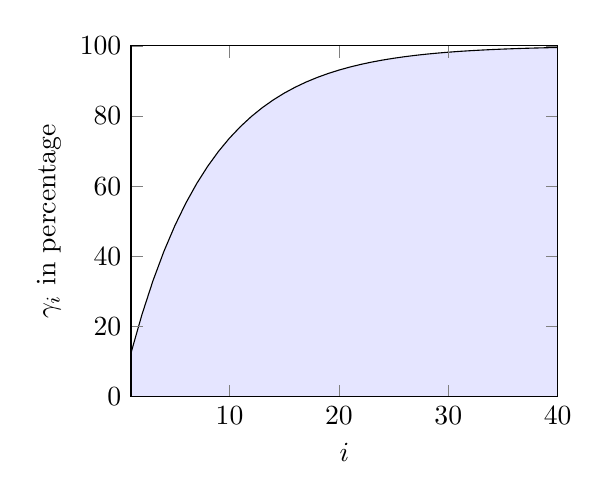
\begin{tikzpicture}
\begin{axis}[
  axis on top,
  xmin=1,
  xmax=40,
  ymin=0,
  ymax=100,
  xlabel={$i$},
  ylabel={$\gamma_i$ in percentage}
  ]
% Calculated by the octave function:
% function y=f(x)
%   y=((8/7).^-x .* (7.^-x.*8.^(x+1)-7))/8;
% endfunction
\addplot[fill=blue!10!white] coordinates {(1,0) (1,12.5) (2,23.437) (3,33.008) (4,41.382) (5,48.709) (6,55.120) (7,60.730) (8,65.639) (9,69.934) (10,73.692) (11,76.981) (12,79.858) (13,82.376) (14,84.579) (15,86.507) (16,88.193) (17,89.669) (18,90.960) (19,92.090) (20,93.079) (21,93.944) (22,94.701) (23,95.364) (24,95.943) (25,96.450) (26,96.894) (27,97.282) (28,97.622) (29,97.919) (30,98.179) (31,98.407) (32,98.606) (33,98.780) (34,98.933) (35,99.066) (36,99.183) (37,99.285) (38,99.374) (39,99.453) (40,99.521) (40,0)};
\end{axis}

\end{tikzpicture}
\end{document}
